\documentclass[hidelinks,12pt]{article}

\usepackage{amsmath}    % need for subequations
\usepackage{graphicx}   % need for figures
\usepackage{verbatim}   % useful for program listings
\usepackage{color}      % use if color is used in text
\usepackage{subfigure}  % use for side-by-side figures
\usepackage{hyperref}   % use for hypertext links, including those to external documents and URLs
\usepackage[
top    = 2.75cm,
bottom = 2.50cm,
left   = 3.00cm,
right  = 2.50cm]{geometry}

\graphicspath{ {./Figures/} }

% don't need the following. simply use defaults
\setlength{\baselineskip}{16.0pt}    % 16 pt usual spacing between lines



\begin{document}
\begin{center}
  {\huge Homework 5}\\
  \vspace{10px}
  
\includegraphics{Logo} \\
  Date of Submission:\\
  February 25, 2019\\
  \vspace{30px}
  \rule{300px}{0.5px} \\
  Thorne Wolfenbarger \\
  \href{mailto:wolfent1@my.erau.edu}{wolfent1@my.erau.edu} \\
  \vspace{30px}
  Submitted to: \\
  Professor Kaela Martin \\
  College of Engineering \\
  \vspace{40px}
  In Partial Fulfillment \\
  of the Requirements of \\
  \vspace{10px}
  AE 313 \\
  Space Mechanics \\
  Spring, 2019 \\
\end{center}

\flushleft \large 1\\
\begin{figure}[!htb]
  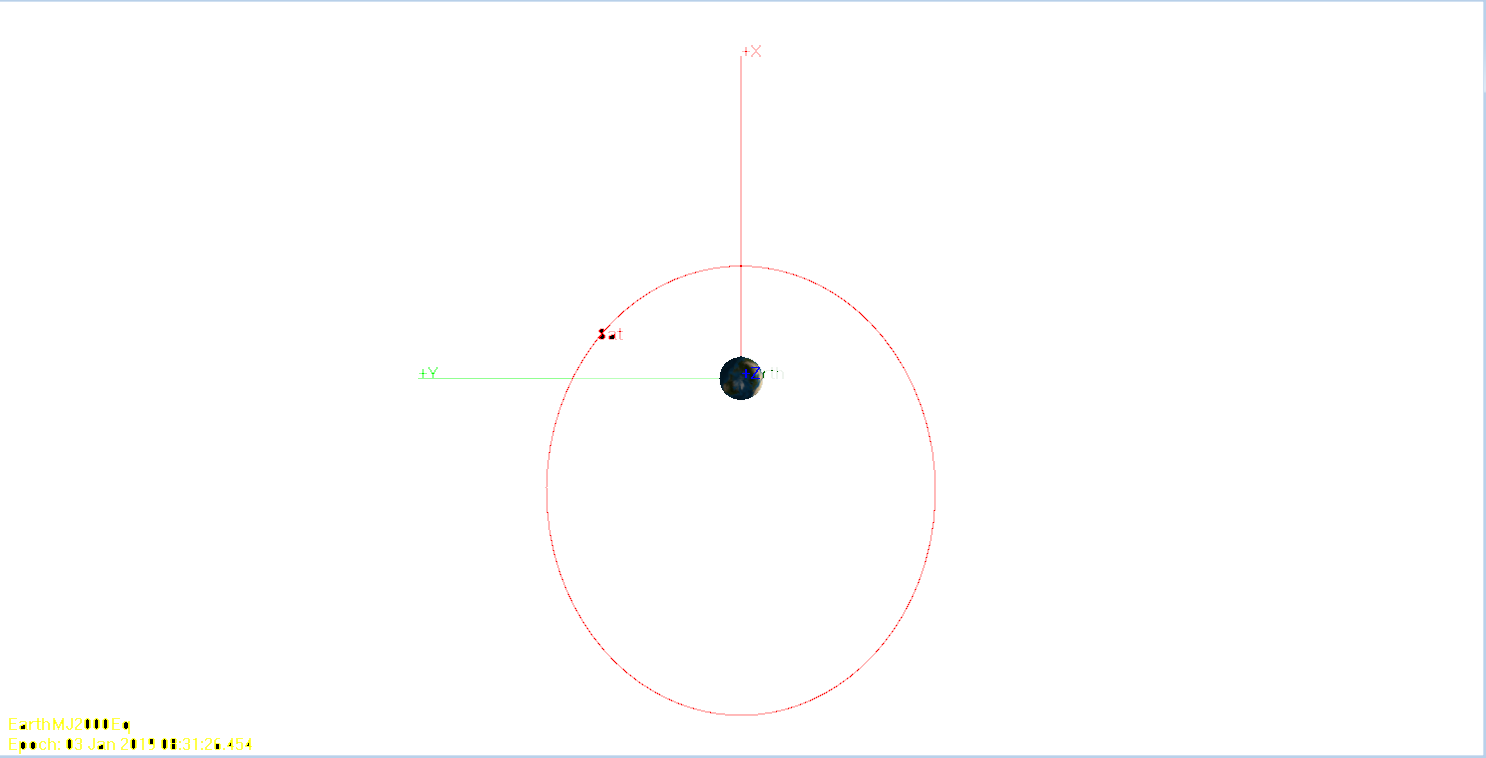
\includegraphics[scale=0.4]{HW4-2}
  \caption{Earth Only Propogator}
  \label{}
\end{figure}

\newpage
\flushleft \large 2\\
\normalsize
\begin{figure}[!htb]
  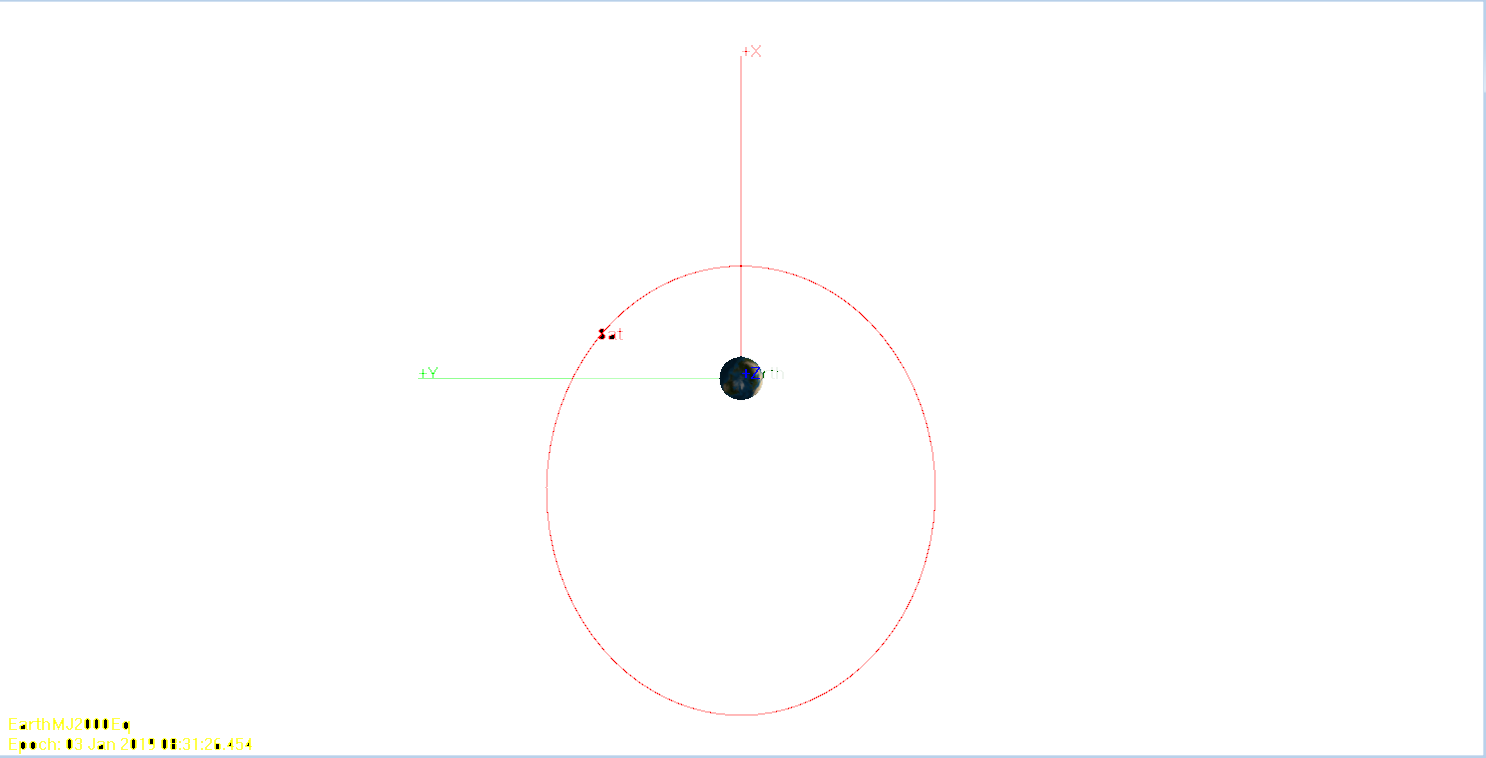
\includegraphics[scale=0.4]{HW4-2}
  \caption{EMS Propogator}
  \label{}
\end{figure}
There is no apparent difference between the satellite's behavior in an Earth system vs an Earth-Moon-Sun system. It does seem reasonable to work with an Earth point mass model due to the fact that in 2-body relative motion each body affects the other like a point mass.

\end{document}
